\section{Setup/Experiment}

The authors use a package called SOCKEYE to parse arbitrary model definitions,
defined with ADL. They then test the models on the WMT and IWSLT datasets.
Models were trained with 6 encoder and 6 decoder layers. Convolution layers all
had kernel sizes of 3 and RNNs used LSTM cells. By testing where attention is
the authors got the following results, BLEU scores. From these scores it is
clear that attention on the upper encoding block is most important, but the
effects aren't that strong. 
\begin{center}
\begin{tabular}{c||c|c}
    Encoder block & IWSLT & WMT'17 \\
    \hline
    upper & $25.4\pm 0.2$ & $27.6 \pm 0.0$\\
    increasing & $25.4\pm 0.1$ & $27.3 \pm 0.1$\\
    decreasing & $25.3 \pm 0.2$ & $27.1 \pm 0.1$
\end{tabular}
\end{center}
In the next experiment the authors adjusted their base RNN and CNN models and
made them more transformer like. It can be seen from the results that the more
transformer like their scores also converge to the transformer BLEU score.
\begin{figure}[ht]
    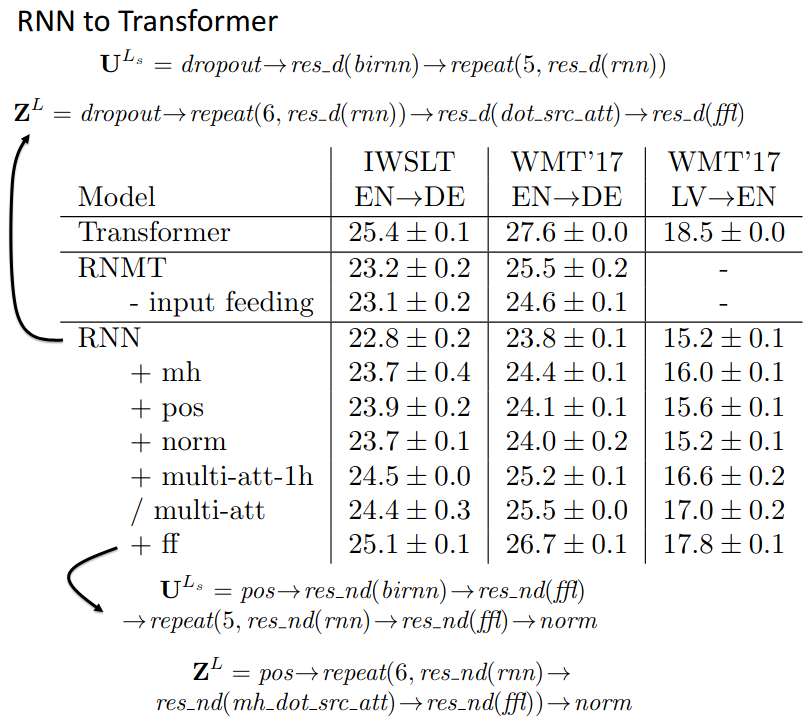
\includegraphics[width=0.45\textwidth]{RNN2Trans.png}
    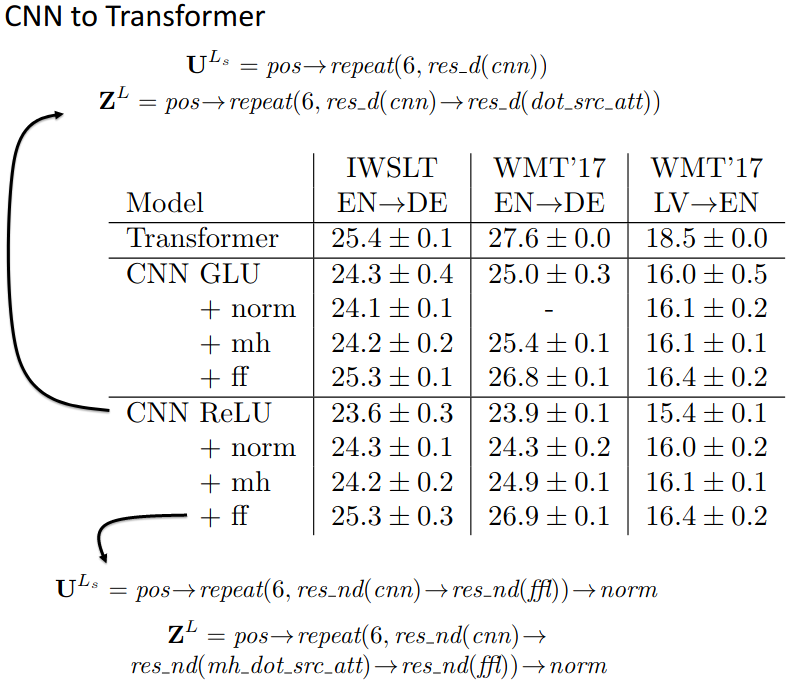
\includegraphics[width=0.45\textwidth]{CNN2Trans.png}
\end{figure}
The last experiment the authors performed was placing attention at different
locations. The results are as follows.
\begin{figure}[ht]
    \center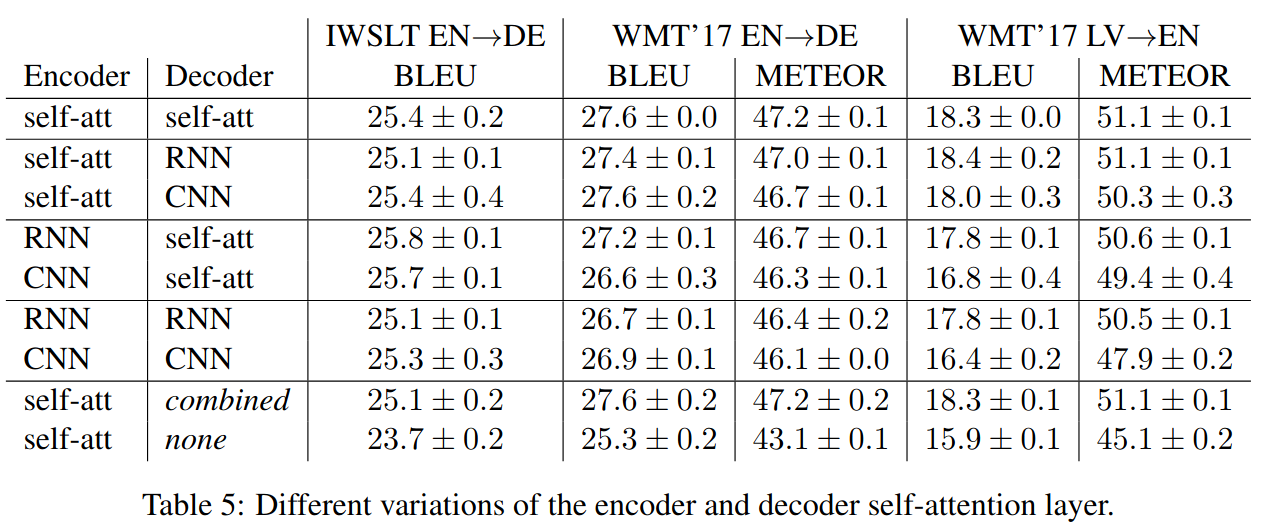
\includegraphics[width=0.7\textwidth]{Variations.png}
\end{figure}
From these results it is clear that self attention on the encoding side is more
influential than on the decoding side. 
